\documentclass{article}
\usepackage[margin=1in]{geometry}
\usepackage{amsmath,amsthm,amssymb}
\usepackage{bbm,enumerate,mathtools}
\usepackage{tikz,pgfplots}
\usepackage{chessboard}
\usepackage[hidelinks]{hyperref}
\usepackage{multicol} % Problem 35
\usepackage{xstring} % Difficulty command
\usetikzlibrary{shapes.geometric}

\newenvironment{question}{\begin{trivlist}\item[\textbf{Question.}]}{\end{trivlist}}
\newenvironment{note}{\begin{trivlist}\item[\textbf{Note.}]}{\end{trivlist}}
\newenvironment{references}{\begin{trivlist}\item[\textbf{References.}]}{\end{trivlist}}
\newenvironment{related}{\begin{trivlist}\item[\textbf{Related.}]\end{trivlist}\begin{enumerate}}{\end{enumerate}}

\newcommand\score[1]{
\pgfmathsetmacro\pgfxa{#1+1}
\tikzstyle{scorestars}=[
  star,
  star points=5,
  star point ratio=2.25,
  draw,
  inner sep=3pt,
  anchor=outer point 5
]
  \begin{tikzpicture}[baseline]
    \draw[opacity=0] (0,-0.5) rectangle (0,0.2); % Workaround for whitespace at the bottom.
    \foreach \i in {1,...,4} {
      \pgfmathparse{(\i<=#1?"yellow":"gray")}
      \edef\starcolor{\pgfmathresult}
      \draw (\i*4.5ex,0) node[name=star\i,scorestars,fill=\starcolor]  {};
    }
  \end{tikzpicture}
}

\newcommand{\difficulty}[1]{%
  \IfEqCase{#1}{%
      {1}{
        
\begin{tikzpicture}[scale=0.7, baseline=0.9mm]%
          \definecolor{slopegreen}{rgb}{0.0, 0.5, 0.0}%
          \fill[slopegreen] (0.5,0.5) circle (0.5);%
        \end{tikzpicture}%
      }%
      {2}{
        
\begin{tikzpicture}[scale=0.7, baseline=0.9mm]%
          \definecolor{slopeblue}{rgb}{0.0, 0.44, 1.00}
          \fill[slopeblue] (0,0) rectangle (1,1);%
        \end{tikzpicture}%
      }%
      {3}{
\begin{tikzpicture}[scale=0.7, baseline=0.9mm]\fill (0,0.5)--(0.5, 0)--(1,0.5)--(0.5,1)--cycle; \end{tikzpicture}}%
      {4}{
\begin{tikzpicture}[scale=0.7, baseline=0.9mm]\fill (0.25,0)--(0,0.5)--(0.25,1)--(0.5,0.5)--cycle; \fill (0.75,0)--(0.5,0.5)--(0.75,1)--(1,0.5)--cycle;\end{tikzpicture}}%
      % you can add more cases here as desired
  }[\PackageError{difficulty}{Undefined difficulty level: #1}{}]%
}%
\newcommand{\rating}[2]{\difficulty{#1}\\\score{#2}\\}


\begin{document}

\rating{2}{2}
There are two popular, essentially identical, iPhone games in the app store:
\textit{AMAZE!!!} and \textit{Roller Splat!}.
The goal of the puzzle is to reach every (white) square in the board---the catch
is that you can only move in as-long-as-possible rook moves.
\begin{figure}[ht!]
  \centering
  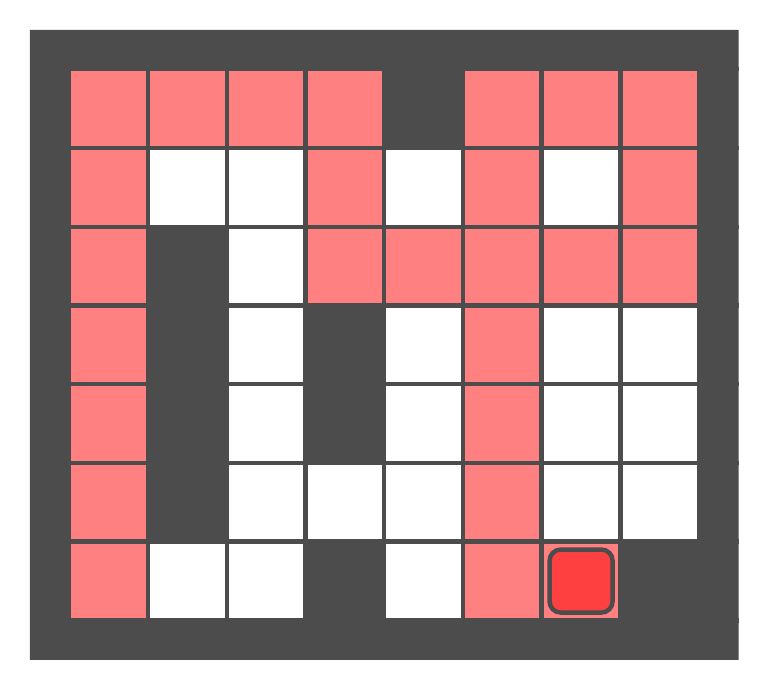
\begin{tikzpicture}
    \draw[line width=27,red!50] (1.5,1)--(1.5,7.5)--(4.5,7.5)--(4.5,5.5)--(8.5,5.5)--(8.5,7.5)--(6.5,7.5)--(6.5,1.5)--(8,1.5);
    \draw[black!70, ultra thick] (0.5,0.5) grid (9.5,8.5);
    \fill[black!70]
      (9.5,1) rectangle (0.5,0.5) rectangle (1,8.5)
      (9,0.5) rectangle (9.5,8.5) rectangle (0.5,8)
      (2,2) rectangle (3,6)
      (4,0.5) rectangle (5,2)
      (4,3) rectangle (5,5)
      (6,8.5) rectangle (5,7)
      (8,0.5) rectangle (9,2)
    ;
    \draw[black!70, ultra thick, rounded corners, fill=red!75] (7.1,1.1) rectangle (7.9,1.9);
  \end{tikzpicture}
  \caption{
    Starting from the lower right corner, the board can be filled using the following $25$ moves: $
      \protect\underbrace{
        \uparrow\rightarrow\downarrow\rightarrow\uparrow\leftarrow\downarrow\rightarrow
      }_\text{illustrated above}
      \uparrow\downarrow\leftarrow\uparrow\leftarrow\rightarrow\downarrow\leftarrow\uparrow\downarrow\leftarrow
    $
  }
\end{figure}

\begin{question}
  How many solvable puzzles exist on an $n \times m$ board?
\end{question}

\begin{related}
  \item What if we only want to count ``primitive'' puzzles---those that cannot
  exist on a smaller board?
  \item What if we count up to symmetries of the rectangle?
  \item Which puzzle requires the greatest number of moves?
  \item What if we do this on a torus? M\"obius strip? More dimensions?
  \item Given some configuration, what is an algorithm to figure out how to solve it?
\end{related}

\end{document}
